\chapter{Background}
% Add maximum likelihood background explanation
% Add Bayesian probability background explanation

\section{Computer Based Tests}
CBT abbreviation
- offers advantages such as being able to display higher quality visuals such as pictures, videos, graphs, etc...
- low paperwork, everything is stored on the computer
- automatic grading, less work for teachers
- generation of statistics is made easier by the fact that the data can be processed by the computer
- nowadays a lot of learning is done on computer systems, and children are used to dealing with computers so assessment through this medium is advantageous. \newline

CBTs are typically "fixed-item" tests where all the students answer the same set of questions,  usually provided by the person responsible for the assessment. This isn't ideal since students can be presented with questions that are too easy or too difficult for them to answer. Consequently, the results of the test won't give a very accurate representation of a student's ability, and for this reason, these types of tests aren't extremely useful. This problem lead to research and the development of computerized adaptive testing (CAT).

\section{Computerized Adaptive Testing}
Computerized adaptive testing (CAT), also called \textit{tailored testing}, is a form of computer-based testing which administers questions (referred to as \textit{items} in the psychometrics literature) of the appropriate difficulty by adapting to the examinee's ability.
For example, if an examinee answers an item correctly, then the next item presented will higher on the difficulty scale. On the other hand, if they answer incorrectly, they will be presented with an item lower on the difficulty scale. \newline

\begin{figure}[H]
\centering
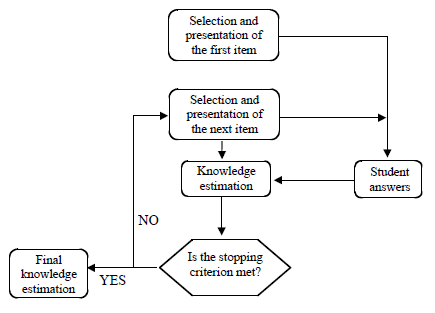
\includegraphics[scale=1]{cat_flowchart}
\caption{Flowchart of an adaptive test. Adapted from SIETTE paper.}
\label{fig:cat_flowchart}
\end{figure}

The flowchart in figure~\ref{fig:cat_flowchart} illustrates the algorithm implemented in computer:
\begin{itemize}
\item[1.] The pool of items that haven't been administered yet is searched to determine the best item to present to the examinee, according to the current estimation of his ability.
\item[2.] The chosen item is presented to the examinee, who then answers it correctly or incorrectly
\item[3.] The ability estimate is updated, based upon all prior answers
\item[4.] Steps 1–3 are repeated until a termination criterion is met
\end{itemize}

Usually, nothing is known about the examinee before administering the first item, so the algorithm is 

 However, it is possible to supply the algorithm with relevant information about the examinees such as previous results or previous estimated abilities.

\begin{itemize}
\item Motivation
\item Explain how it works
\item Algorithm picture/flowchart
\item Advantages and disadvantages of CAT
%\item (Last sentence) usually based on IRT -> nice lead in to next section ....... In general, CATs use IRT (Section 2.2) as a response model.
\end{itemize}

Advantages include
- precise scores for most test takers
- requires less items to be administered before arriving at an equally accurate score, in comparison to static multiple choice tests
- like any computer based test adaptive tests may show results immediately after testing, no grading having to be done by teachers, so saves time and money.

Disadvantages include 
- the need for a large bank of calibrated items to cater to all ability levels.
- Items are administered one by one, so once an answer to the item has been given there is no turning back. No skipping questions either.


%http://edglossary.org/computer-adaptive-test/
\begin{itemize}
\item Students can be presented with questions/exercises that are either too easy or too difficult.
\item CAT is a solution to this problem as it automatically chooses the exercises of the appropriate difficulty level for the students.
\item Based on IRT for item selection
\item Evaluation of CAT
\end{itemize}

\section{Probabilistic Test Theory}
\subsection{Maximum Likelihood}
% Add maximum likelihood background explanation
% Conditional probability quick overview?
% Add Bayesian probability background explanation
% Bayesian networks
% Latent variables ?

IRT is based on the idea that the probability of a correct/keyed response to an item is a mathematical function of person and item parameters. 

\begin{itemize}
\item Calculates the probability of a particular student answering a specific item correctly.
\item Different IRT models: One-Parameter Logistic (1-PL), Two-Parameter Logistic (2-PL), Three-Parameter Logistic (3-PL). Refers to the number of parameters used in the model. Parameters are: 

\begin{itemize}
\item[-] item difficulty parameter (\textit{b})
\item[-] item discrimination parameter (\textit{a})
\item[-] chance/guessing parameter (\textit{c})
\end{itemize}

\item Item Characteristic Curve, i.e. probability distribution
\end{itemize}

\subsection{Bayes probability theory}

\subsection{Item Response Theory}
For these reasons, Item response theory (IRT) has seen frequent usage when it comes to CATs....We present the different models developed to predict the probability of a correct or incorrect response to a particular item.
\subsubsection{The one-parameter logistic model}
dfsdfsdf
\subsubsection{The two-parameter logistic model}
dfsdfsdf
\subsubsection{The three-parameter logistic model}
dfsdfsdf
